\univlogo

{\Huge April 8}\vspace{5mm}

\section*{After-class assignments}

\subsection*{4.5}

Derive a gradient descent training rule for a single unit with output o, where

\begin{equation}
\begin{aligned}
    o=w_0+w_1x_1+w_1x_1^2+\dots+w_nx_n+w_nx_n^2
\end{aligned}
\end{equation}

Answer:
\begin{equation}
\begin{aligned}
    E(\vec{w})&=\cfrac{1}{2}\sum_{d\in D}(t_d-o_d)^2\\
    \cfrac{\partial E}{\partial w_i}&=\sum_{d\in D}(t_d-o_d)\cdot(x_i+x_i^2)\\
    \therefore \Delta w_i&=-\eta\cfrac{\partial E}{\partial w_i}=\eta\sum_{d\in D}(t_d-o_d)(-x_i-x_i^2)
\end{aligned}
\end{equation}

\subsection*{4.6}

Explain informally why the delta training rule in Equation(4.10) is only an approximation to the true gradient descent rule of Equation(4.7).

\begin{equation}
\begin{aligned}
    \Delta w_i&=\eta(t-o)x_i &(4.10)\\
    \Delta w_i&=\eta\sum_{d\in D}(t_d-o_d)x_{id} &(4.7)    \nonumber
\end{aligned}
\end{equation}

Answer:
Batch gradient descent uses the whole data set to determine the $\Delta w_i$, while stocastic gradient descent uses single random point.

Equation (4.10) corresponds to incremental gradient descent in which weights 
are updated after seeing each of the examples, while Equation (4.7) corresponds 
to true gradient descent in which the weights are updated after seeing all the 
examples once.

\subsection*{4.7}

Consider a two-layer feedforward ANN with two inputs $a$ and $b$, one hidden unit $c$, and one output unit $d$. This network has five weights ($w$, $w_{cb}$, $w_{eb}$, $w_{d}$, $w_{dc}$, $w_{dO}$), where $w_{xo}$ represents the threshold weight for unit $x$. Initialize these weights to the values (.1, .l, .l, .l, .1), then give their values after each of the first two training iterations of the BACKPROPAGATION algorithm. Assume learning rate $\eta=.3$, momentum $\alpha=0.9$, incremental weight updates, and the following training examples:

\begin{equation}
\begin{matrix}
    a&b&d\\
    1&0&1\\
    0&1&0   \nonumber
\end{matrix}
\end{equation}

Answer:

\begin{figure}[H]
    \centering
    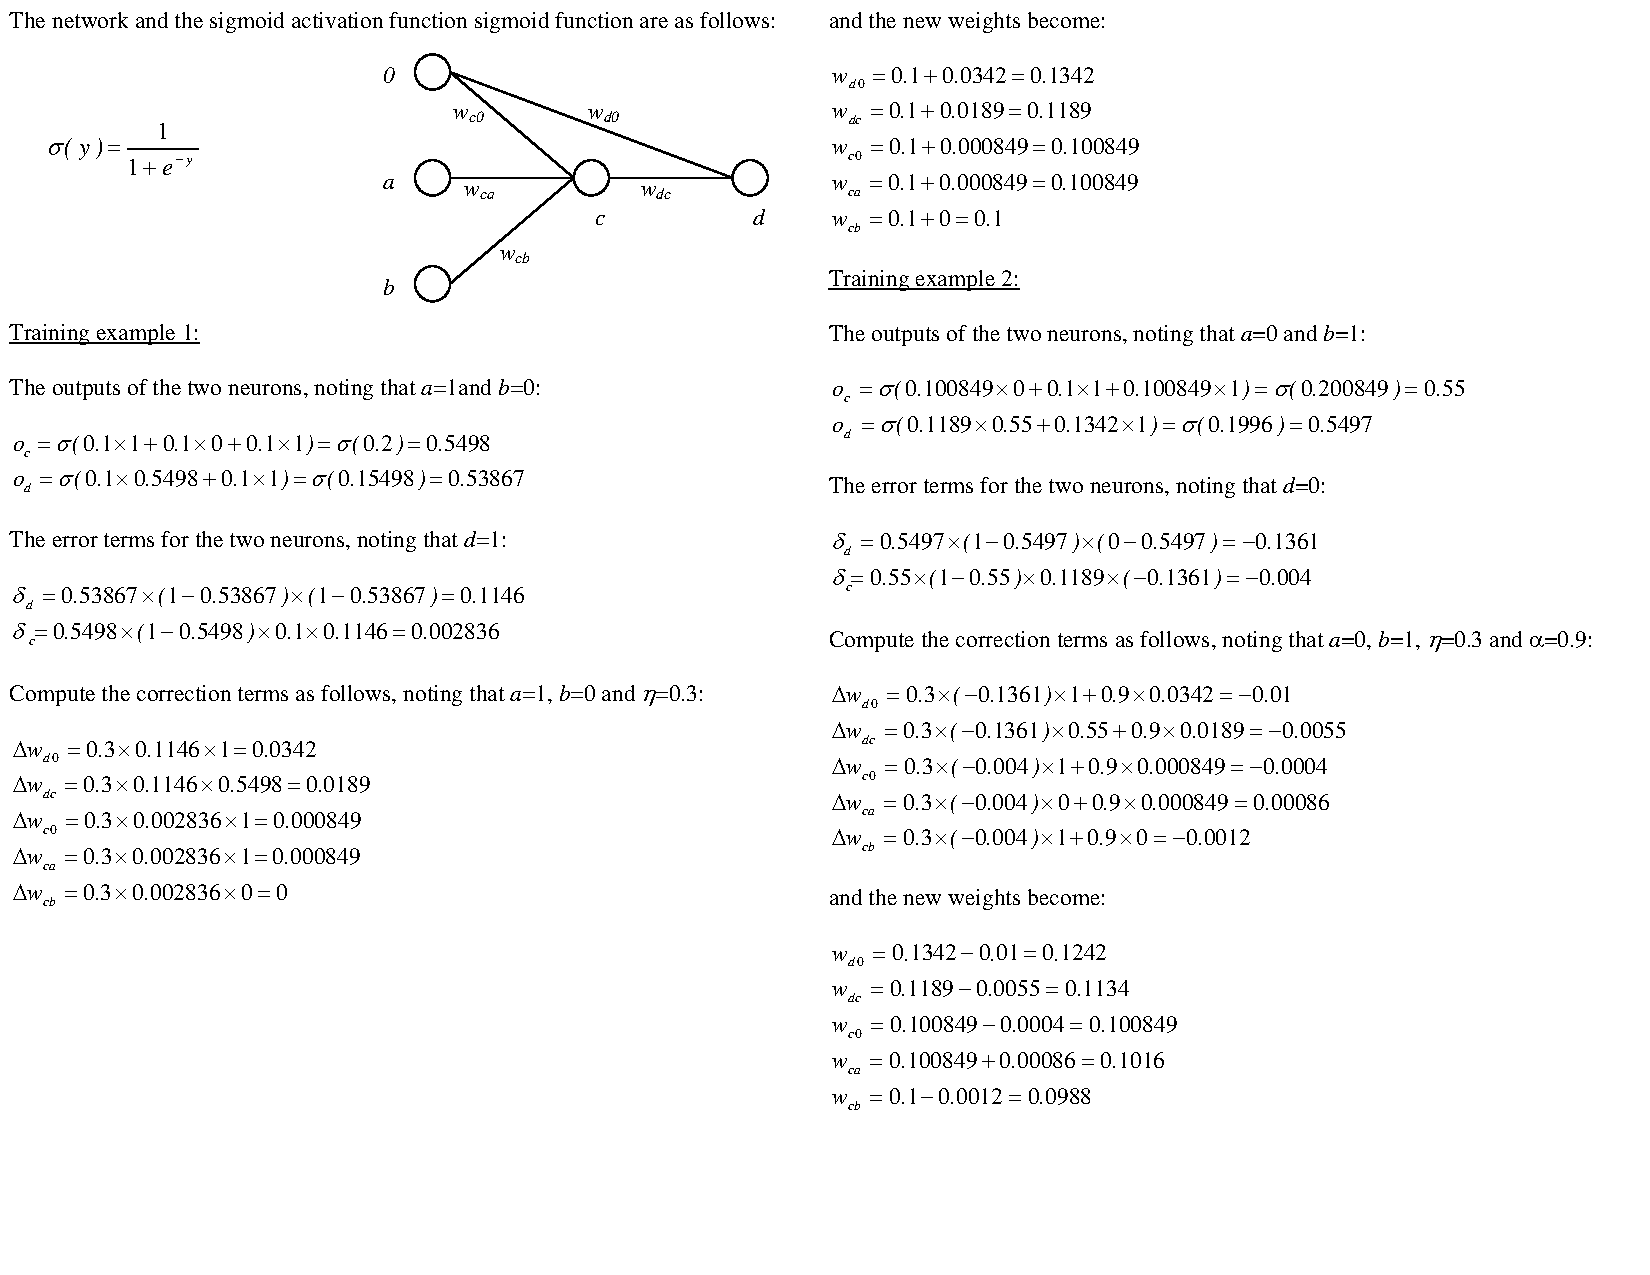
\includegraphics[width=1\textwidth]{./2023April/solution4_7.pdf}
    \caption{}
    \label{solution4_7}
\end{figure}
